\documentclass[a4paper, 12pt]{article}

%Абзацный отступ

\usepackage{indentfirst}

%Рисунки

\usepackage{graphicx}
\usepackage{wrapfig}

%Гиперссылки и работа с цветом

\usepackage{hyperref}
\usepackage[rgb]{xcolor}
\hypersetup{			%Гиперссылки
	colorlinks=true, 	%false: ссылки в рамках
	urlcolor=blue		%на URL
}

%Русский язык

\usepackage[T2A]{fontenc}		%кодировка
\usepackage[utf8]{inputenc}		%кодировка исходного текста
\usepackage[english, russian]{babel}	%локализация и переносы


%Математика

\usepackage{amsmath, amsfonts, amssymb, amsthm, mathtools, mathrsfs}

%Пакет с градусом

\usepackage{gensymb}

\author{Штрайх Роберт}
\title{Работа 3.5.1. Изучение плазмы газового разряда в неоне}
\date{today}

\begin{document}
\begin{titlepage}
	\centering
	\vspace{5cm}
	{\scshape\LARGE Московский физико-технический институт \par}
	\vspace{4cm}
	{\scshape\Large Лабораторная работа №3.5.1 \par}
	\vspace{1cm}
	{\huge\bfseries Изучение плазмы газового разряда в неоне\par}
	\vspace{1cm}
	\vfill
\begin{flushright}
	{\Large выполнил студент 006 группы ФЭФМ}\par
	\vspace{0.3cm}
	{\Large Штрайх Роберт}
\end{flushright}
	

	\vfill

% Bottom of the page
	Долгопрудный, 2021 г.
\end{titlepage}

\newpage

\textbf{Цель работы:} изучение вольт-амперной характеристики тлеющего разряда: изучение свойств плазмы методом зондовых характеристик.

\textbf{В работе используются:} стеклянная газоразрядная трубка, наполненная изотопом неона, высоковольтный источник питания, источник питания постоянного тока, делитель напряжения, резистор, потенциометр, амперметры, вольтметры, переключатели.

\section{Теоретическое введение}
\subsection*{Плазма}
В ионизированном газе поле ионов <<экранируется>> электронами. Для поля $\mathbf{E}$ и плотности $\rho$ электрического заряда
$$
\text{div}~\mathbf{E} = 4 \pi \rho,
$$
а с учётом сферической симметрии и $\mathbf{E} = -\text{grad}~\varphi$:
\begin{equation}
\dfrac{d^2 \varphi}{dr^2}+\dfrac{2}{r}\dfrac{d\varphi}{dr}=-4\pi \rho.
\end{equation}
Плотности заряда электронов и ионов (которые мы считаем бесконечно тяжёлыми и поэтому неподвижными)
\begin{equation}
\begin{array}{c}
\rho_e = -ne \cdot \exp\left(\dfrac{e\varphi}{kT_e}\right),\\
\rho_i = ne.
\end{array}
\end{equation}
Тогда из $(1)$ в предположении $\dfrac{e\varphi}{kT_e} \ll 1$ получим
\begin{equation}
\varphi = \dfrac{Ze}{r}e^{-r/r_D},
\end{equation}
где $r_D = \sqrt{\dfrac{kT_e}{4\pi n e^2}}$ -- \textit{радиус Дебая}. Среднее число ионов в сфере такого радиуса 
\begin{wrapfigure}{r}{4cm}
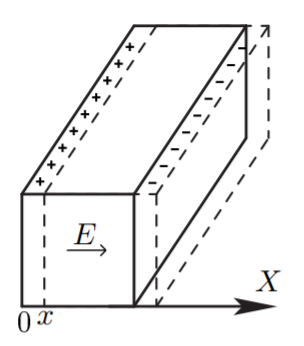
\includegraphics[scale=0.5]{2.png}
\end{wrapfigure}  
\begin{equation}
N_D = n\dfrac{4}{3}\pi r_D^2.
\end{equation}
Теперь выделим параллелепипед с плотностью $n$ электронов, сместим их на $x$. Возникнут поверхностные заряды $\sigma = nex$, поле от которых будет придавать электронам ускорение:
$$
\dfrac{d^2x}{dt^2}=-\dfrac{eE}{m}=-\dfrac{4\pi n e^2}{m}x.
$$ 
Отсюда получаем \textit{плазменную (ленгмюровскую) частоту} колебаний электронов:
\begin{equation}
\omega_p = \sqrt{\dfrac{4\pi ne^2}{m}}.
\end{equation}
\subsection*{Одиночный зонд}
При внесении в плазму уединённого проводника -- \textit{зонда} -- с потенциалом, изначально равным потенциалу точки плазмы, в которую его помещают, на него поступают токи электроннов и ионов:
\begin{equation}
\begin{array}{c}
I_{e0} = \dfrac{n \langle v_e \rangle}{4}eS,\\
I_{i0} = \dfrac{n \langle v_i \rangle}{4}eS,
\end{array}
\end{equation}
где $\langle v_e \rangle$ и $\langle v_i \rangle$ -- средние скорости электронов и ионов, $S$ -- площадь зонда, $n$ -- плотность электронов и ионов. Скорости электронов много больше скорости ионов, поэтому $I_{i0} \ll I_{e0}$. Зонд будет заряжаться до некоторого равновестного напряжения $-U_f$ -- \textit{плавающего потенциала}.\\
\begin{wrapfigure}{r}{5.5cm}
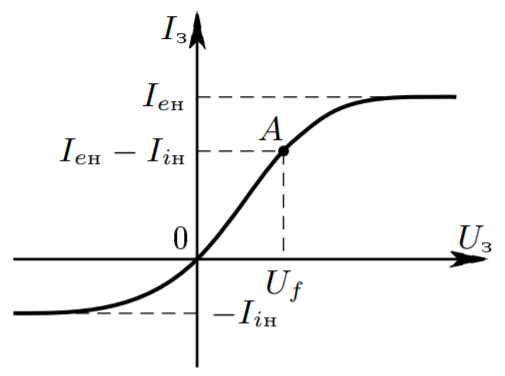
\includegraphics[scale=0.5]{3.png}
\end{wrapfigure}  
В равновесии ионный ток мало меняется, а электронный имеет вид
$$
I_e = I_0 \exp\left( -\dfrac{eU_f}{kT_e} \right).
$$
Будем подавать потенциал $U_\text{з}$ на зонд и снимать значение зондового тока $I_\text{з}$. Максимальное значение тока $I_{e\text{н}}$ -- электронный ток насыщения, а минимальное $I_{i\text{н}}$ -- ионный ток насыщения. Значение из эмпирической формулы Бомона:
\begin{equation}
I_{i\text{н}} = 0.4 neS \sqrt{\dfrac{2kT_e}{m_i}}.
\end{equation}
\subsection*{Двойной зонд}
Двойной зонд -- система из двух одинаковых зондов, расположенных на небольшом расстоянии друг от друга, между которыми создаётся разность потенциалов, меньшая $U_f$. Рассчитаем ток между ними вблизи $I=0$. При небольших разностях потенциалов ионные токи на оба зонда близки к току насыщения и компенсируют друг друга, а значит величина результирующего тока полностью связана с разностью электронных токов. Пусть потенциалы на зондах
$$
U_1 = -U_f + \Delta U_1,
$$
$$
U_2 = -U_f + \Delta U_2.
$$
Между зондами $U = U_2 - U_1 = \Delta U_2 - \Delta U_1$.
Через первый электрод
\begin{equation}
I_1 = I_{i\text{н}} + I_{e1} = I_{i\text{н}} - \dfrac{1}{4}neS\langle v_e\rangle \exp\left(-\dfrac{eU_f}{kT_e}\right)\exp\left(\dfrac{e\Delta U_1}{kT_e}\right)=I_{i\text{н}}\left(1 - \exp\left( \dfrac{e\Delta U_1}{kT_e} \right)\right).
\end{equation}
Аналогично через второй получим
\begin{equation}
I_2 = I_{i\text{н}}\left(1 - \exp\left( \dfrac{e\Delta U_2}{kT_e} \right)\right)
\end{equation}
  
Из $(7)$ и $(8)$ с учётом последовательного соединение зондов ($I_1 = -I_2 = I)$:
$$
\Delta U_1= \dfrac{kT_e}{e}\text{ln}\left(1 - \dfrac{I}{I_{i\text{н}}}\right)
$$
$$
\Delta U_2= \dfrac{kT_e}{e}\text{ln}\left(1 + \dfrac{I}{I_{i\text{н}}}\right)
$$

Тогда итоговые формулы для разности потенциалов и тока

\begin{equation}
U = \dfrac{kT_e}{e}\text{ln}\dfrac{1 - I/I_{i\text{н}}}{1 + I/I_{i\text{н}}}, 
I = I_{i\text{н}} \text{th}\dfrac{eU}{2kT_e}.
\end{equation}
Реальная зависимость выглядит несколько иначе и описывается формулой 
\begin{wrapfigure}{l}{7cm}
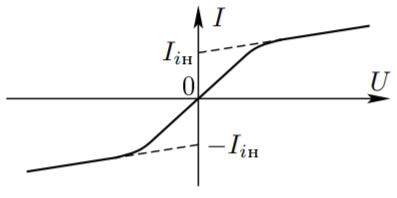
\includegraphics[scale=0.8]{4.png}
\vspace{+30pt}
\end{wrapfigure}
\begin{equation}
I = I_{i\text{н}} \text{th}\dfrac{eU}{2kT_e} + AU.
\end{equation}
Из этой формулы можно найти формулу для $T_e$: для $U=0$ мы найдём $I_{i\text{н}}$, продифференцируем в точке $U=0$ и с учётом $\text{th}~\alpha \approx \alpha$ при малых $\alpha$ и $A\rightarrow 0$ получим:
\begin{equation}
kT_e = \dfrac{1}{2}\dfrac{eI_{i\text{н}}}{\dfrac{dI}{dU}|_{U=0}}.
\end{equation}

\newpage
\section{Экспериментальная установка}

\begin{figure}[h]
\begin{center}
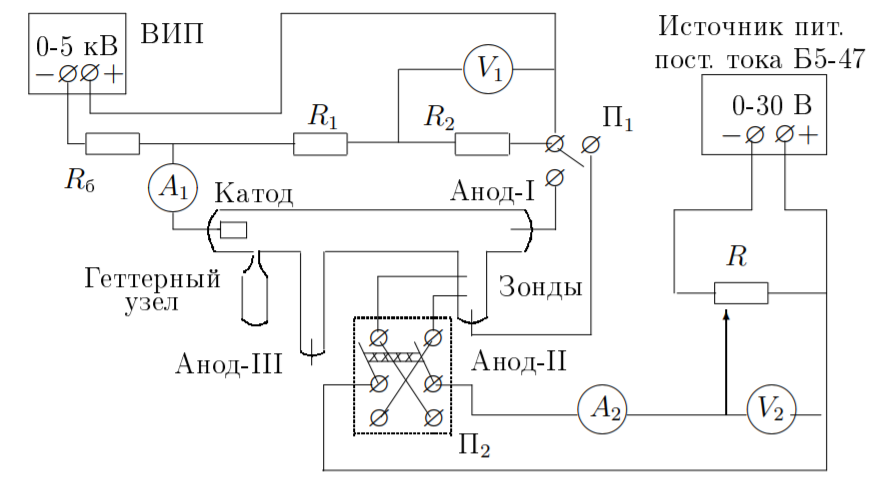
\includegraphics[width=1\textwidth]{Схема_установки}
\end{center}
\caption{Схема экспериментальной установки} \label{Установка}
\end{figure}

Схема установки для исследования плазмы газового разряда в неоне представлена на рис. \ref{Установка}. Стеклянная газоразрядная трубка имеет холодный (не нагреваемый)полый катод, три анода и \textit{геттерный узел} -- стеклянный балон, на внутреннюю поверхность которого напылена газопоглощающая плёнка (\textit{геттер}). Трубка наполнена изотопом неона $^{22}$Ne при давлении 2 мм рт. ст. Катод и один из анодов (I или II) с помощью переключателя $\Pi_1$ подключаются через балластный резистор $R_{б}$ ($\sim$ 500 кОм) к регулируемому высоковольтному источнику питания (ВИП) с выходным напряжением до нескольких киловольт. 

При подключении к ВИП анода-I между ним и катодом возникает газовый разряд. Ток разряда измеряется миллиамперметром $A_1$, а падение напряжения на разрядной трубке -- вольтметром $V_1$, подключённым к трубке через высокоомный (несколько десятков МОм) делитель напряжения с коэффициентом $(R_1+R_2)/R_2$.

При подключении к ВИП анода-II разряд возникает в пространстве между катодом и анодом-II, где находится двойной зонд, используемый для диагностики плазмы положительного столба. Зонды изготовлены из молибденовой проволоки диаметром $d$ и имеют длину $l$. Они подключены к источнику питания через потенциометр $R$. Переключатель $\Pi_2$ позволяет изменять полярность напряжения на зондах. Величина напряжения на зондах изменяется с помощью дискретного переключателя <<$V$>> выходного напряжения источника питания и потенциометра $R$, а измеряется вольтметром $V_2$. Для измерения зондового тока используется микроамперметр $A_2$. Анод-III в нашей работе не используется.

\section{Ход работы}

Измерим вольт-амперную характеристику разряда и данные занесём в таблицу \ref{ВАХ}:


\begin{table}[h]
\caption{ВАХ разряда}
\begin{tabular}{|l|l|l|l|l|l|l|l|l|l|l|l|}
\hline
$I$, мА & 0,8   & 1,2   & 1,6   & 2      & 2,4   & 2,8    & 3,2   & 3,6 & 4     & 4,4   & 4,8    \\ \hline
$U$, В  & 344,2 & 334,3 & 297,6 & 231,82 & 205,5 & 197,5  & 191,2 & 180 & 171,2 & 166,6 & 163    \\ \hline
$I$, мА & 4,8   & 4,4   & 4     & 3,6    & 3,2   & 2,8    & 2,4   & 2   & 1,6   & 1,2   & 0,8    \\ \hline
$U$, В  & 163   & 166,6 & 171,8 & 180,3  & 191,1 & 194,36 & 204,3 & 226 & 296,5 & 331,8 & 342,96 \\ \hline
\end{tabular}
\label{ВАХ}
\end{table}

По данным таблицы построим график \ref{VAH_graph}.
Оценим максимальное дифференциальное сопротивление заряда:

\[R_\text{диф} = dU/dI\]

$R_\text{диф} = (-18,3 \pm 0,2)\cdot10^3$ Ом

Параметры зонда: d = 0.2 мм, l = 5.2 мм
Измерим его ВАХ при фиксированных токах разряда $I_p$. Занесём данные в таблицы \ref{Zond1} -- \ref{Zond3}:

\begin{table}[h]
\caption{I = 1.5 мА}
\small
\begin{tabular}{|l|l|l|l|l|l|l|l|l|l|l|l|}
\hline
$I$, мкА & 27,78 & 26,84 & 25,88  & 24,89  & 23,57  & 21,5  & 19,16 & 16      & 11,8   & 6,48   & 0,25   \\ \hline
$U$, В   & 25    & 22    & 19     & 16     & 13     & 10    & 8     & 6       & 4      & 2      & 0      \\ \hline
$I$, мкА & 0,25  & -6,19 & -11,81 & -16,32 & -19,84 & -22,4 & -24,7 & -26,026 & -27,11 & -28,13 & -29,07 \\ \hline
$U$, В   & 0     & -2    & -4     & -6     & -8     & -10   & -13   & -16     & -19    & -22    & -25    \\ \hline
\end{tabular}
\label{Zond1}
\end{table}

\begin{table}[h]
\caption{I = 3 мА}
\small
\begin{tabular}{|l|l|l|l|l|l|l|l|l|l|l|l|}
\hline
$I$, мкА & 58,06 & 56,41  & 54,79  & 53     & 50,62 & 46,16  & 41,28  & 34,58  & 25,76 & 14,8   & 3,34   \\ \hline
$U$, В   & 25    & 22     & 19     & 16     & 13    & 10     & 8      & 6      & 4     & 2      & 0      \\ \hline
$I$, мкА & -2,79 & -13,53 & -24,82 & -34,34 & -42,2 & -47,47 & -52,35 & -55,33 & -57,2 & -58,36 & -60,66 \\ \hline
$U$, В   & 0     & -2     & -4     & -6     & -8    & -10    & -13    & -16    & -19   & -22    & -25    \\ \hline
\end{tabular}
\label{Zond2}
\end{table}

\begin{table}[h!]
\caption{I = 5 мА}
\footnotesize
\begin{tabular}{|l|l|l|l|l|l|l|l|l|l|l|l|}
\hline
$I$, мкА & 108,58 & 106,34 & 103,53 & 99,88  & 93,84 & 84,74  & 75,68  & 64,19   & 49,15  & 32,88   & 18,92   \\ \hline
$U$, В   & 25     & 22     & 19     & 16     & 13    & 10     & 8      & 6       & 4      & 2       & 0       \\ \hline
$I$, мкА & -15    & -32,71 & -50    & -65,15 & -77,8 & -88,03 & -98,21 & -104,92 & -109,4 & -112,57 & -115,31 \\ \hline
$U$, В   & 0      & -2     & -4     & -6     & -8    & -10    & -13    & -16     & -19    & -22     & -25     \\ \hline
\end{tabular}
\label{Zond3}
\end{table}

По данным таблиц построим зондовые характеристики $I(U)$.

По каждой из зондовых характеристик (\ref{Zond1_graph} -- \ref{Zond3_graph}) определим ионный ток насыщения $I_{in}$ по пересечению асимптот к графику с осью координат.

\begin{table}[h]
\caption{Токи насыщения}
\begin{center}
\begin{tabular}{|l|l|l|l|}
\hline
    & I=1.5 мА & I=3 мА & I=5 мА \\ \hline
$I_{in}$, мкА & $18,57 \pm 0.2$  & $39,71 \pm 0.1$ & $71,23 \pm 0.2$  \\ \hline
\end{tabular}
\end{center}
\label{Iin}
\end{table}

По каждой из зондовых характеристик определим наклон характеристики $(dI/dU)_{U=0}$ (рис. \ref{Zond1_graph} -- \ref{Zond3_graph}).

\begin{table}[h]
\caption{Наклоны характеристики}
\begin{center}
\begin{tabular}{|l|l|l|l|}
\hline
    & I=1.5 мА & I=3 мА & I=5 мА \\ \hline
$dI/dU$, мкА/В & $3.24 \pm 1.03$  & $6.77 \pm 1.41$ & $16.36 \pm 2.09$  \\ \hline
\end{tabular}
\end{center}
\label{Iin}
\end{table}

Определим температуру электронов $T_e$:

\[kT_e = \frac{1}{2}\frac{eI_{in}}{\frac{dI}{dU}}\]

\begin{table}[h!]
\caption{Температура электронов}
\begin{center}
\begin{tabular}{|l|l|l|l|}
\hline
    & I=1.5 мА & I=3 мА & I=5 мА \\ \hline
$T_e$, эВ & $2.87 \pm 0.86$  & $2.93 \pm 0.59$ & $2.18 \pm 0.39$  \\ \hline
\end{tabular}
\end{center}
\label{Te}
\end{table}

Рассчитаем концентрацию электронов в плазме:

\[I_{in} = 0.4n_eeS\sqrt{\frac{2kT_e}{m_i}}\]

$S = \pi \cdot d \cdot l$ -- площадь поверхности зонда.

$m_i = 22 \cdot 1.66 \cdot 10^{-27}$ кг -- масса иона неона

\begin{table}[h!]
\caption{Концентрация электронов}
\begin{center}
\begin{tabular}{|l|l|l|l|}
\hline
    & I=1.5 мА & I=3 мА & I=5 мА \\ \hline
$n_e \cdot 10^{16}, \text{м}^{-3}$ & $1.75 \pm 0.23$  & $3.72 \pm 0.29$ & $7.73 \pm 0.56$  \\ \hline
\end{tabular}
\end{center}
\label{n_e}
\end{table}

Рассчитаем плазменную частоту колебаний электронов:

\[\omega_p = \sqrt{\frac{4\pi n_ee^2}{m_e}}\]

\begin{table}[h!]
\caption{Частота колебаний}
\begin{center}
\begin{tabular}{|l|l|l|l|}
\hline
    & I=1.5 мА & I=3 мА & I=5 мА \\ \hline
$\omega_p \cdot 10^9, c^{-1}$ & $7.4 \pm 0.5$  & $10.8 \pm 0.7$ & $155.7 \pm 7.1$  \\ \hline
\end{tabular}
\end{center}
\label{w_p}
\end{table}

Рассчитаем электронную поляризационную длину $r_{De}$:

\[r_{De} = \sqrt{\frac{kT_e}{4\pi n_ee^2}}\text{ см}\]

\begin{table}[h!]
\caption{Электронная поляризационная длина}
\begin{center}
\begin{tabular}{|l|l|l|l|}
\hline
    & I=1.5 мА & I=3 мА & I=5 мА \\ \hline
$r_{De} \cdot 10^{-3}$, см & $9.61 \pm 1.14$  & $6.59 \pm 0.65$ & $4.57 \pm 0.35$  \\ \hline
\end{tabular}
\end{center}
\label{r_De}
\end{table}

Рассчитаем дебаевский радиус экранирования $r_D$:

\[r_{D} = \sqrt{\frac{kT_i}{4\pi n_ee^2}}\text{ см}\]

\begin{table}[h!]
\caption{Дебаевский радиус экранирования}
\begin{center}
\begin{tabular}{|l|l|l|l|}
\hline
    & I=1.5 мА & I=3 мА & I=5 мА \\ \hline
$r_{D} \cdot 10^{-4}$, см & $9.04 \pm 0.48$  & $6.20 \pm 0.27$ & $4.30 \pm 0.13$  \\ \hline
\end{tabular}
\end{center}
\label{r_D}
\end{table}

\newpage
Оценим среднее число ионов в дебаевской сфере:

\[N_D = \frac{4}{3}\pi n_er_D^3\]

\[N_D \sim 10^{-2}\]

Оценим степень ионизации плазмы, считая $P \simeq 2$ торр:

\[\alpha = n_e\frac{kT_e}{P}\]

\begin{table}[h!]
\caption{Степень ионизации плазмы}
\begin{center}
\begin{tabular}{|l|l|l|l|}
\hline
    & I=1.5 мА & I=3 мА & I=5 мА \\ \hline
$\alpha \cdot 10^{-7}$ & $2.7 \pm 0.5$  & $5.8 \pm 1.3$ & $12.0 \pm 2.7$  \\ \hline
\end{tabular}
\end{center}
\label{alpha}
\end{table}

Построим графики зависимостей $n_e(I)$,
$T_e(I)$ (рис. \ref{n_e(I)} и рис. \ref{T_e(I)})

\newpage
\section{Выводы}

\begin{enumerate}
\item Изучили вольт-амперную характеристику тлеющего заряда, изучили свойства плазмы методом зондовых характеристик;
\item Рассчитали важные характеристики плазмы: плазменную частоту электронов $\omega_p$,
электронную поляризационную длину $r_{De}$ и дебаевский радиус экранирования $r_D$;
\item Получили зависимости $n_e(I)$,
$T_e(I)$.
\end{enumerate}

\newpage
\section{Приложение}

\begin{figure}[h!]
\begin{center}
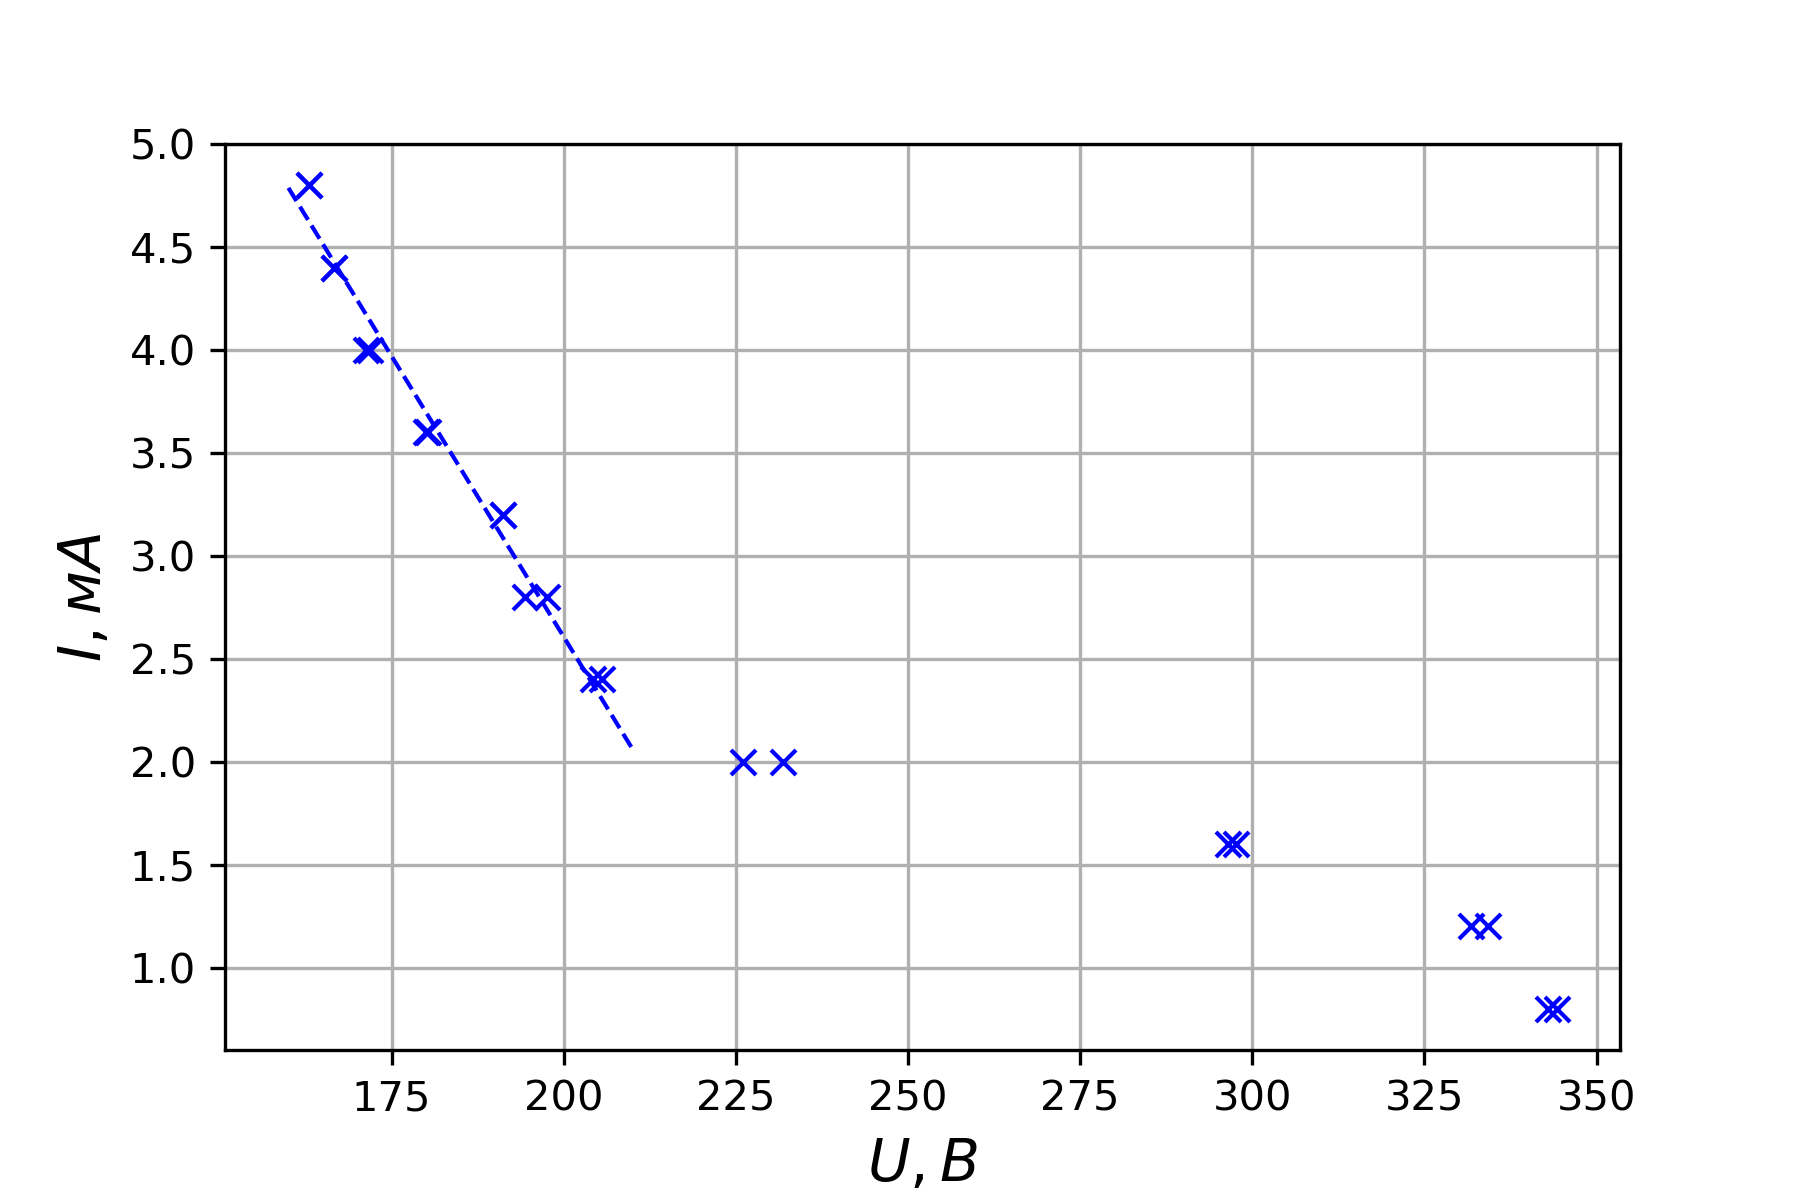
\includegraphics{VAH.png}
\end{center}
\caption{ВАХ разряда}
\label{VAH_graph}
\end{figure}

\begin{figure}[h!]
\begin{center}
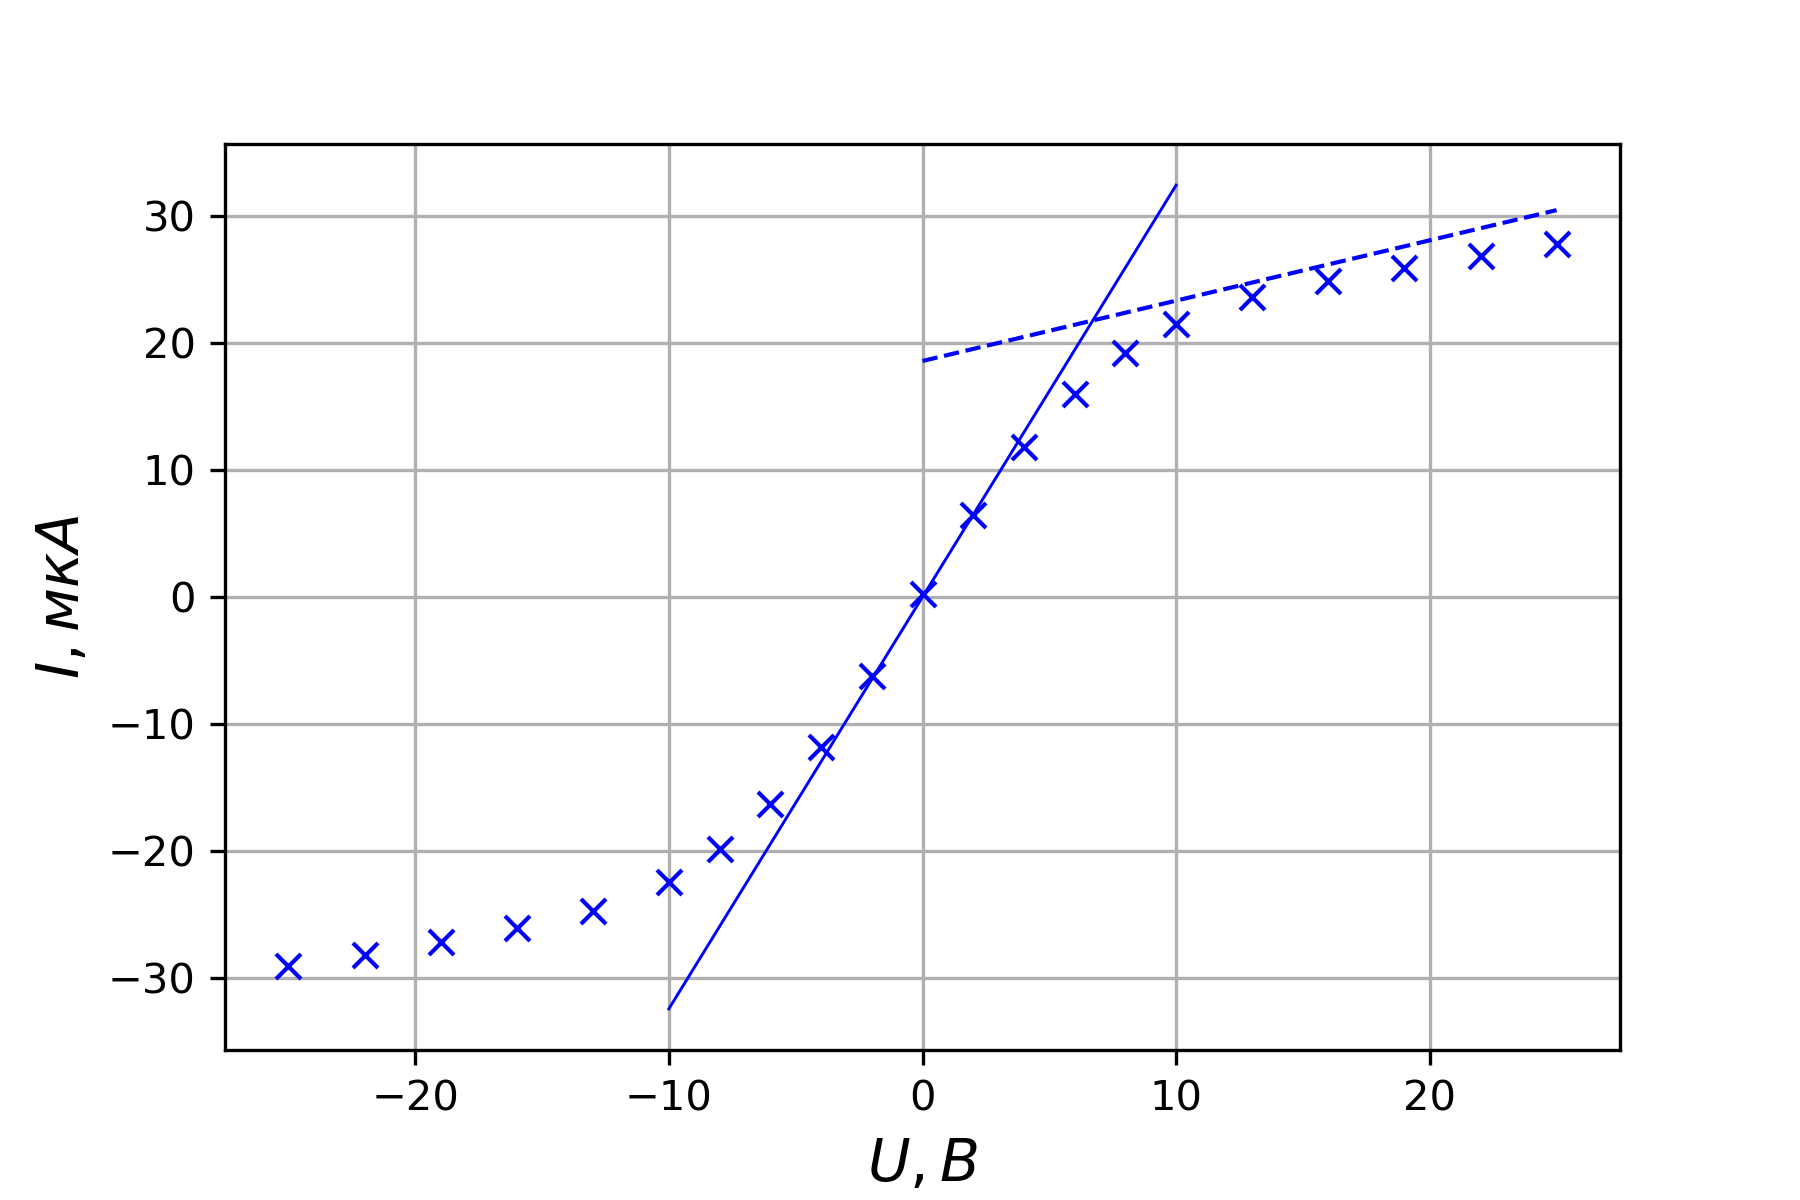
\includegraphics{Zond1.png}
\end{center}
\caption{Зондовая характеристика для I = 1.5 мА}
\label{Zond1_graph}
\end{figure}

\begin{figure}[h!]
\begin{center}
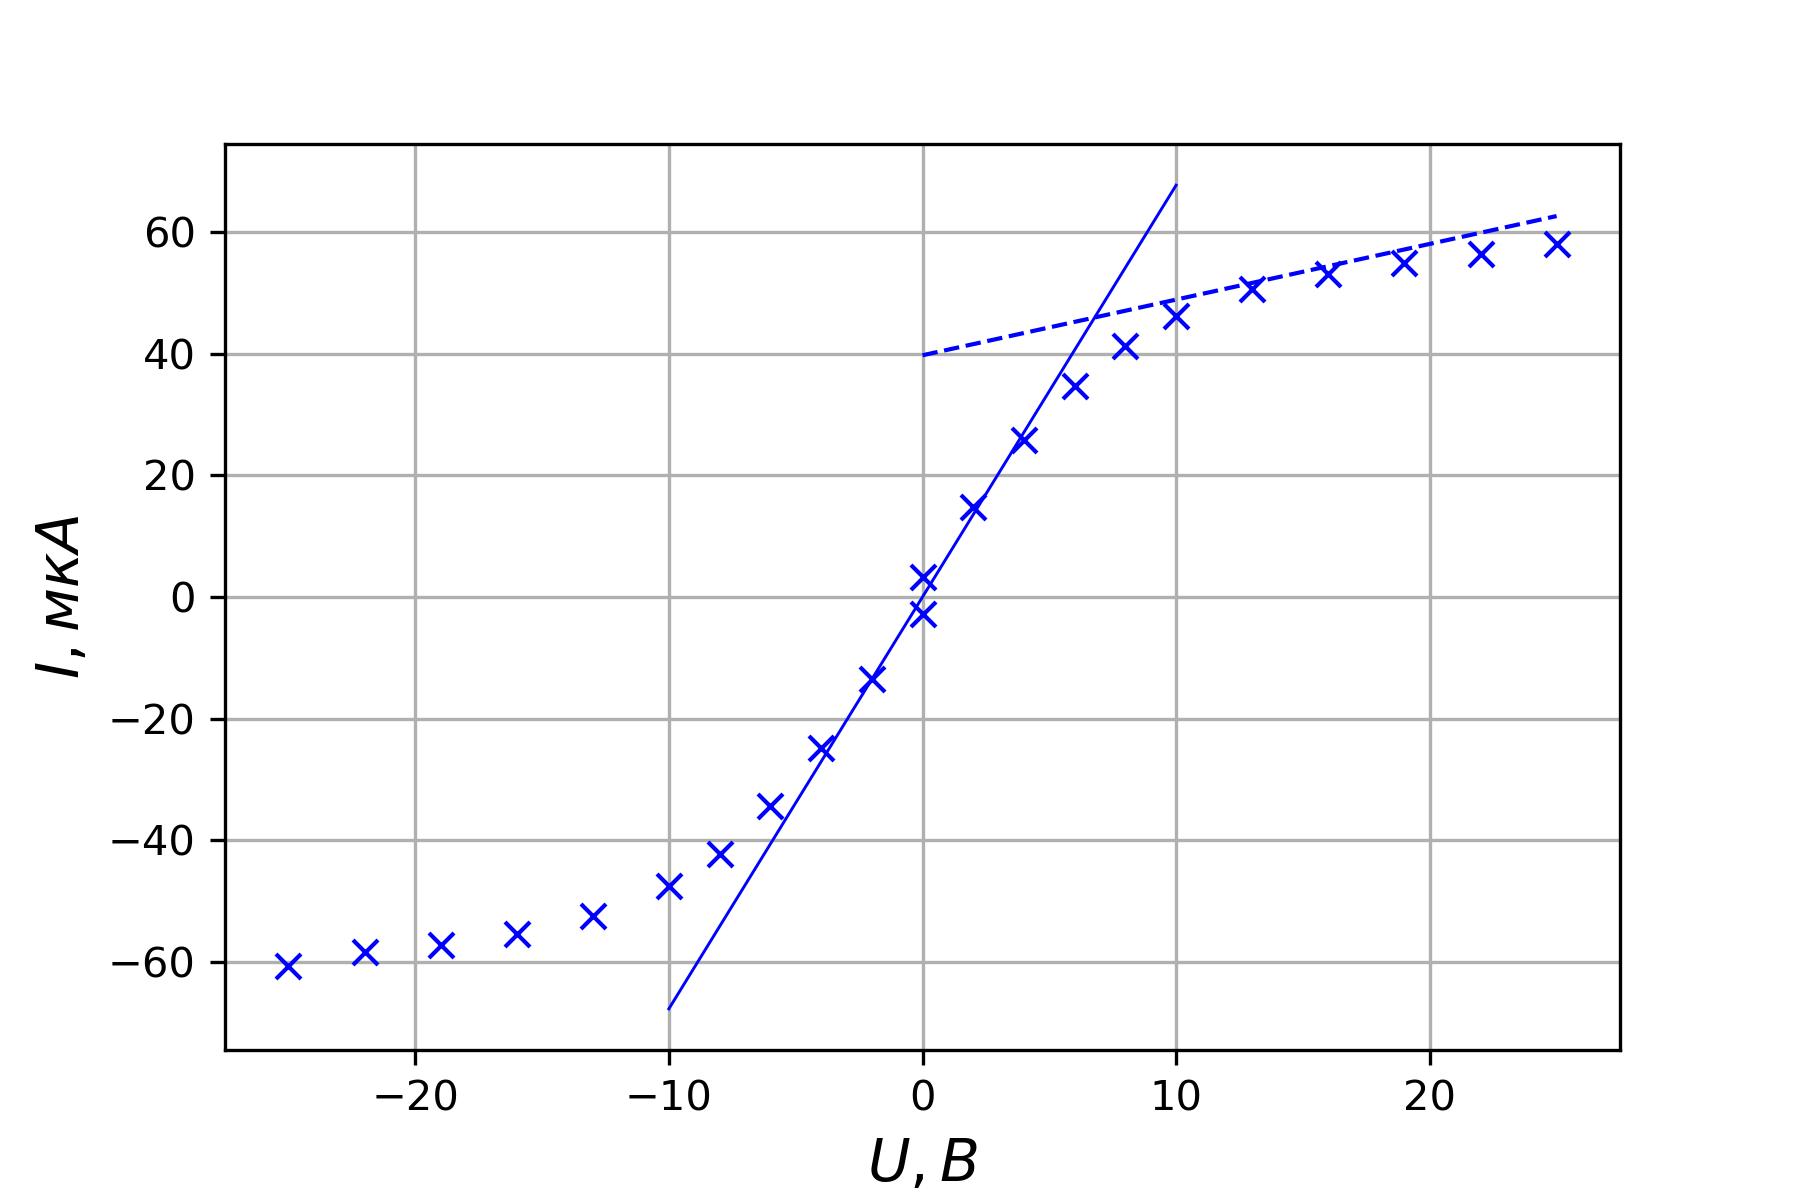
\includegraphics{Zond2.png}
\end{center}
\caption{Зондовая характеристика для I = 3 мА}
\label{Zond2_graph}
\end{figure}

\begin{figure}[h!]
\begin{center}
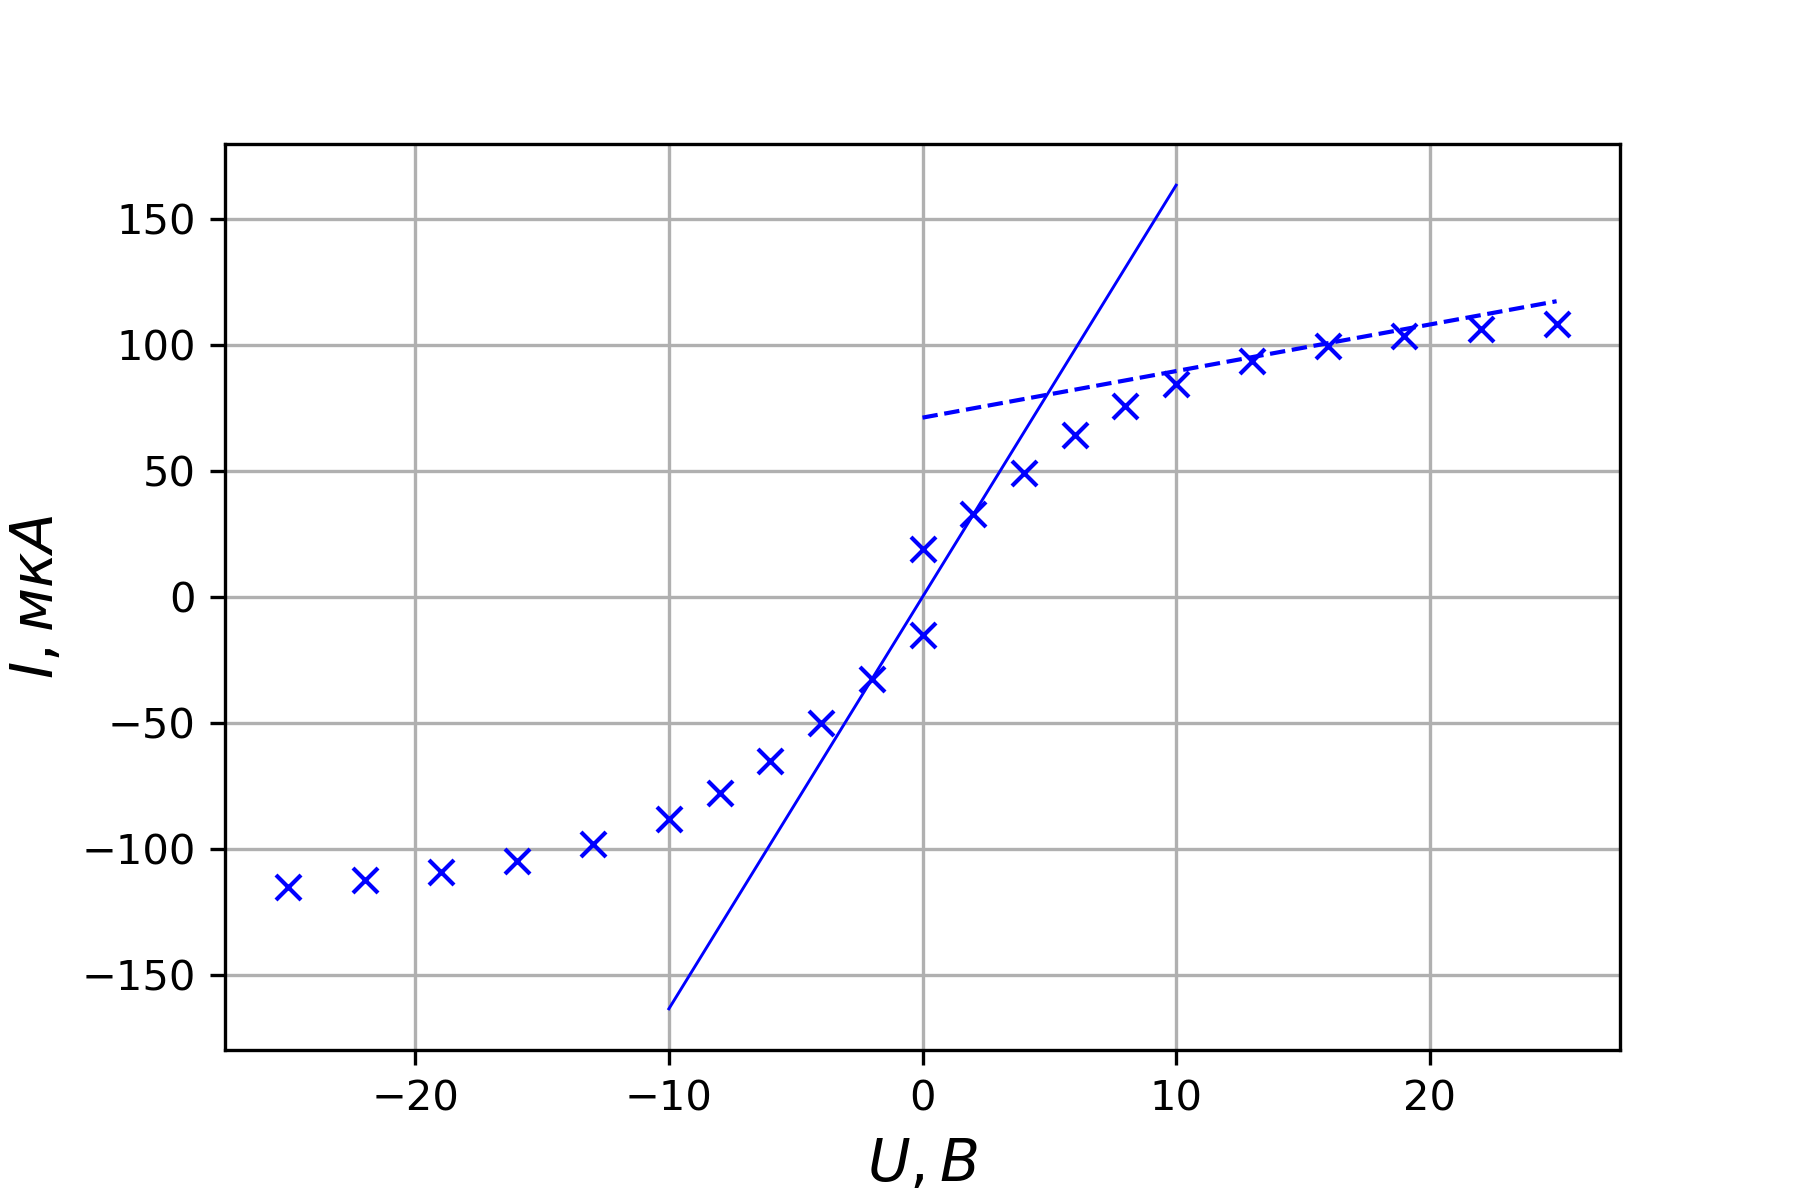
\includegraphics{Zond3.png}
\end{center}
\caption{Зондовая характеристика для I = 5 мА}
\label{Zond3_graph}
\end{figure}

\begin{figure}[h!]
\begin{center}
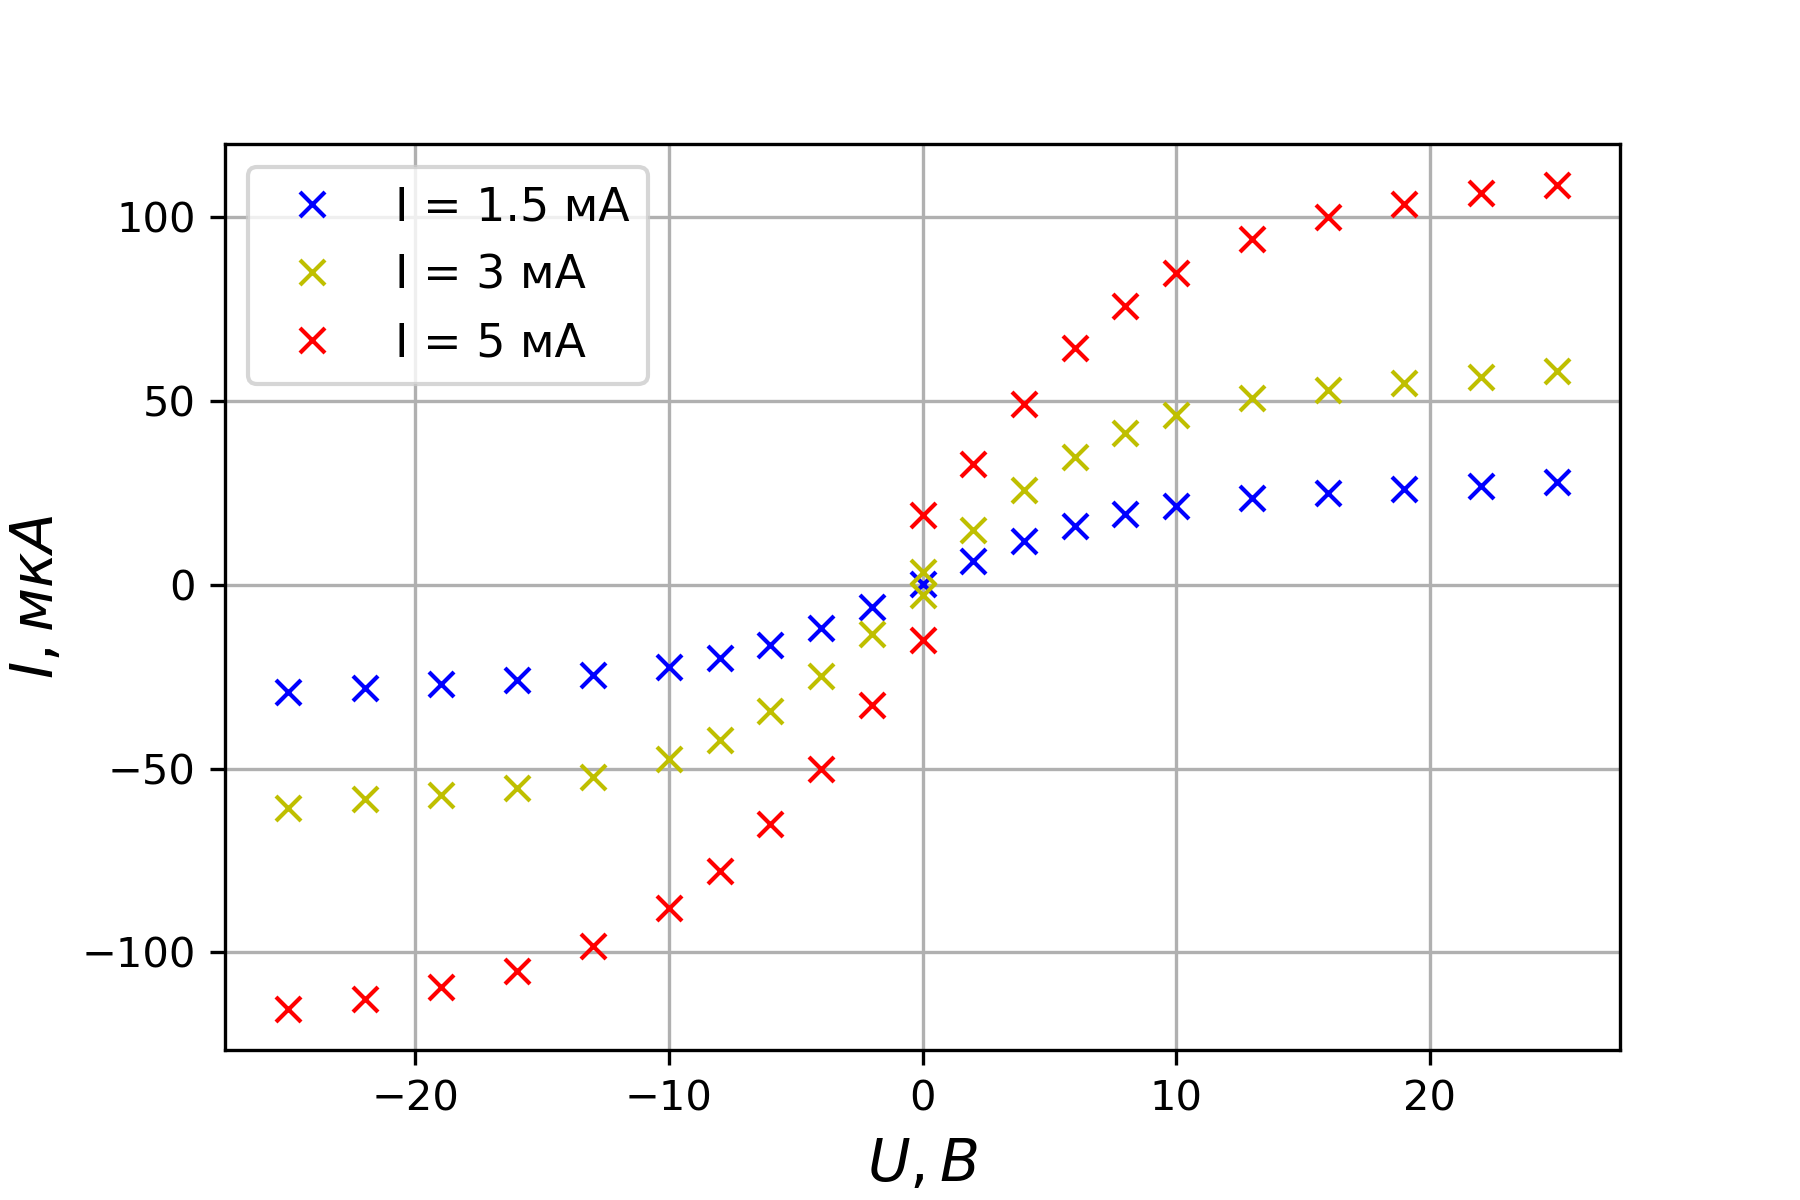
\includegraphics{Zond_all.png}
\end{center}
\caption{Зондовые характеристики}
\label{Zond_all_graph}
\end{figure}

\begin{figure}[h!]
\begin{center}
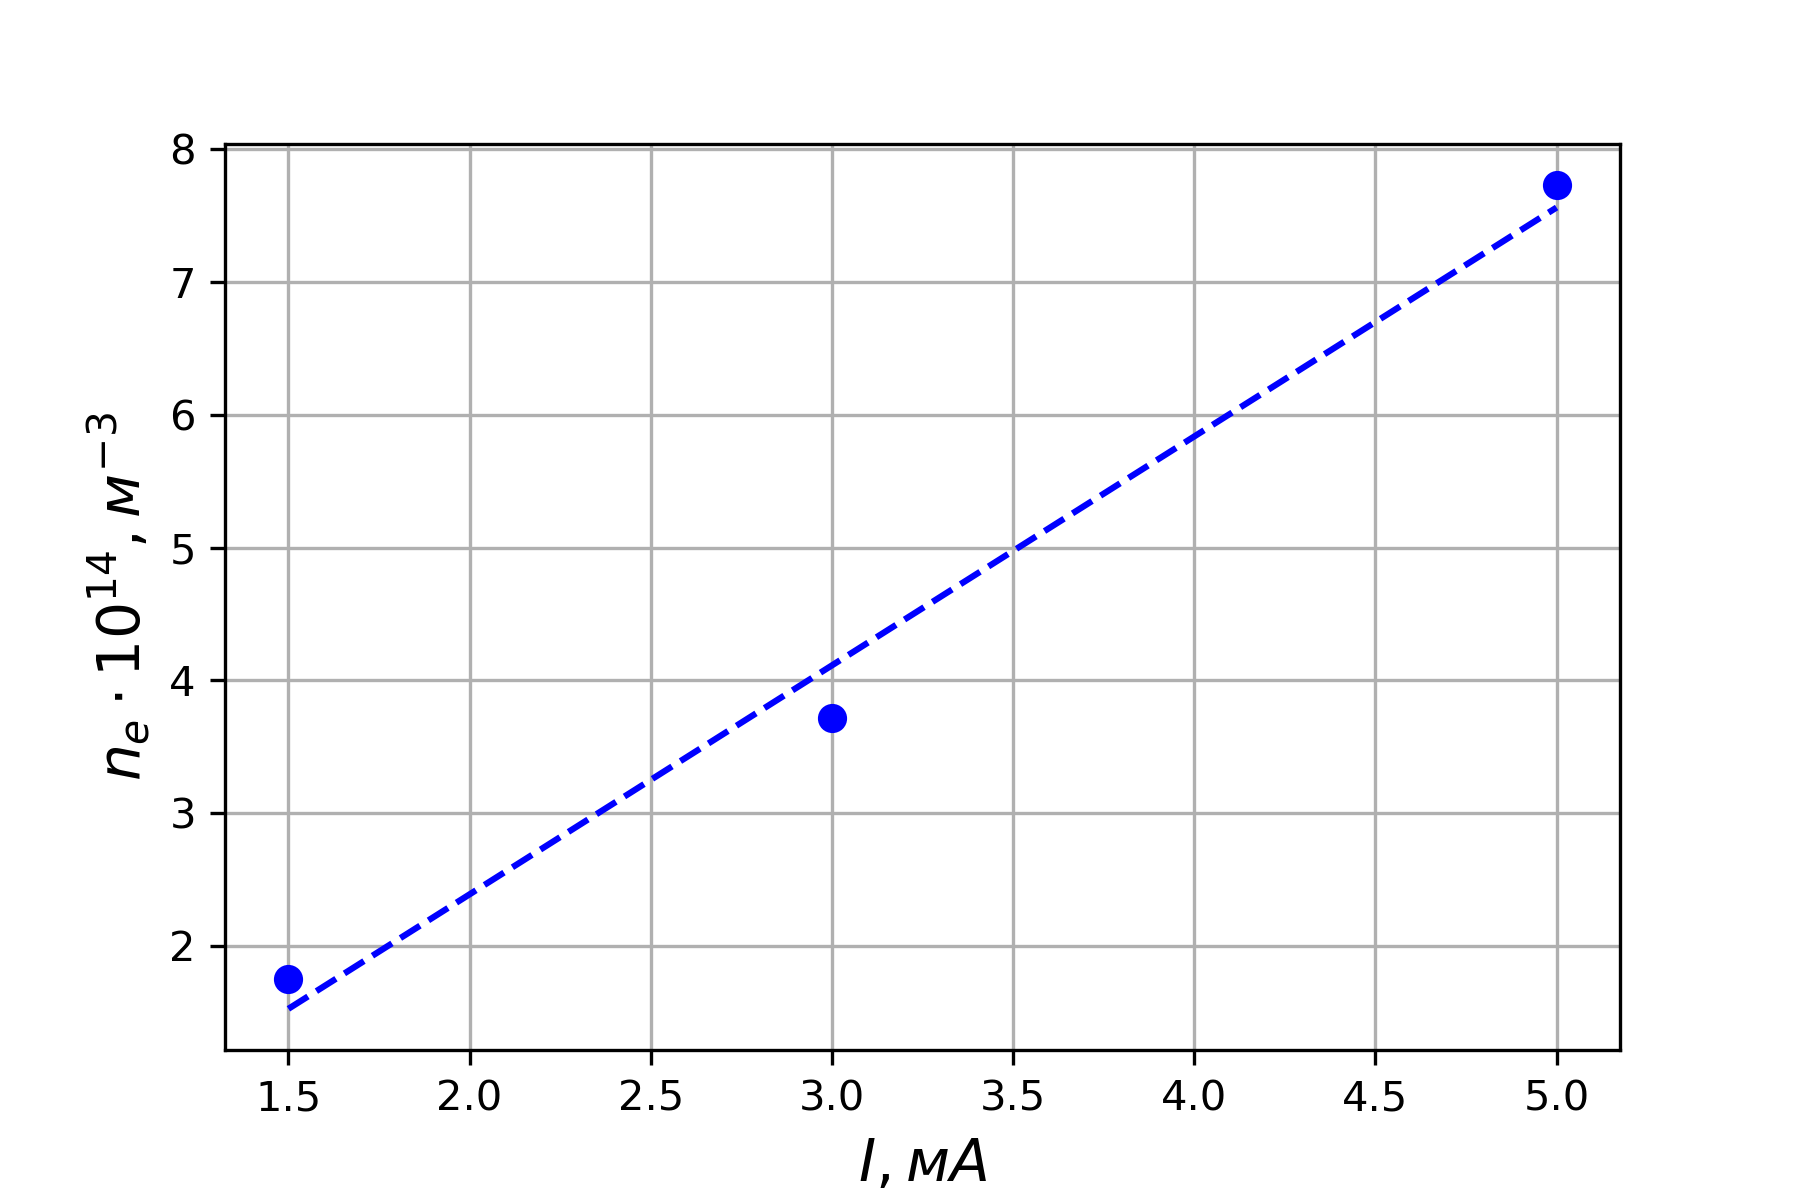
\includegraphics{n_e(Ip).png}
\end{center}
\caption{Зависимость $n_e(I)$}
\label{n_e(I)}
\end{figure}

\begin{figure}[h!]
\begin{center}
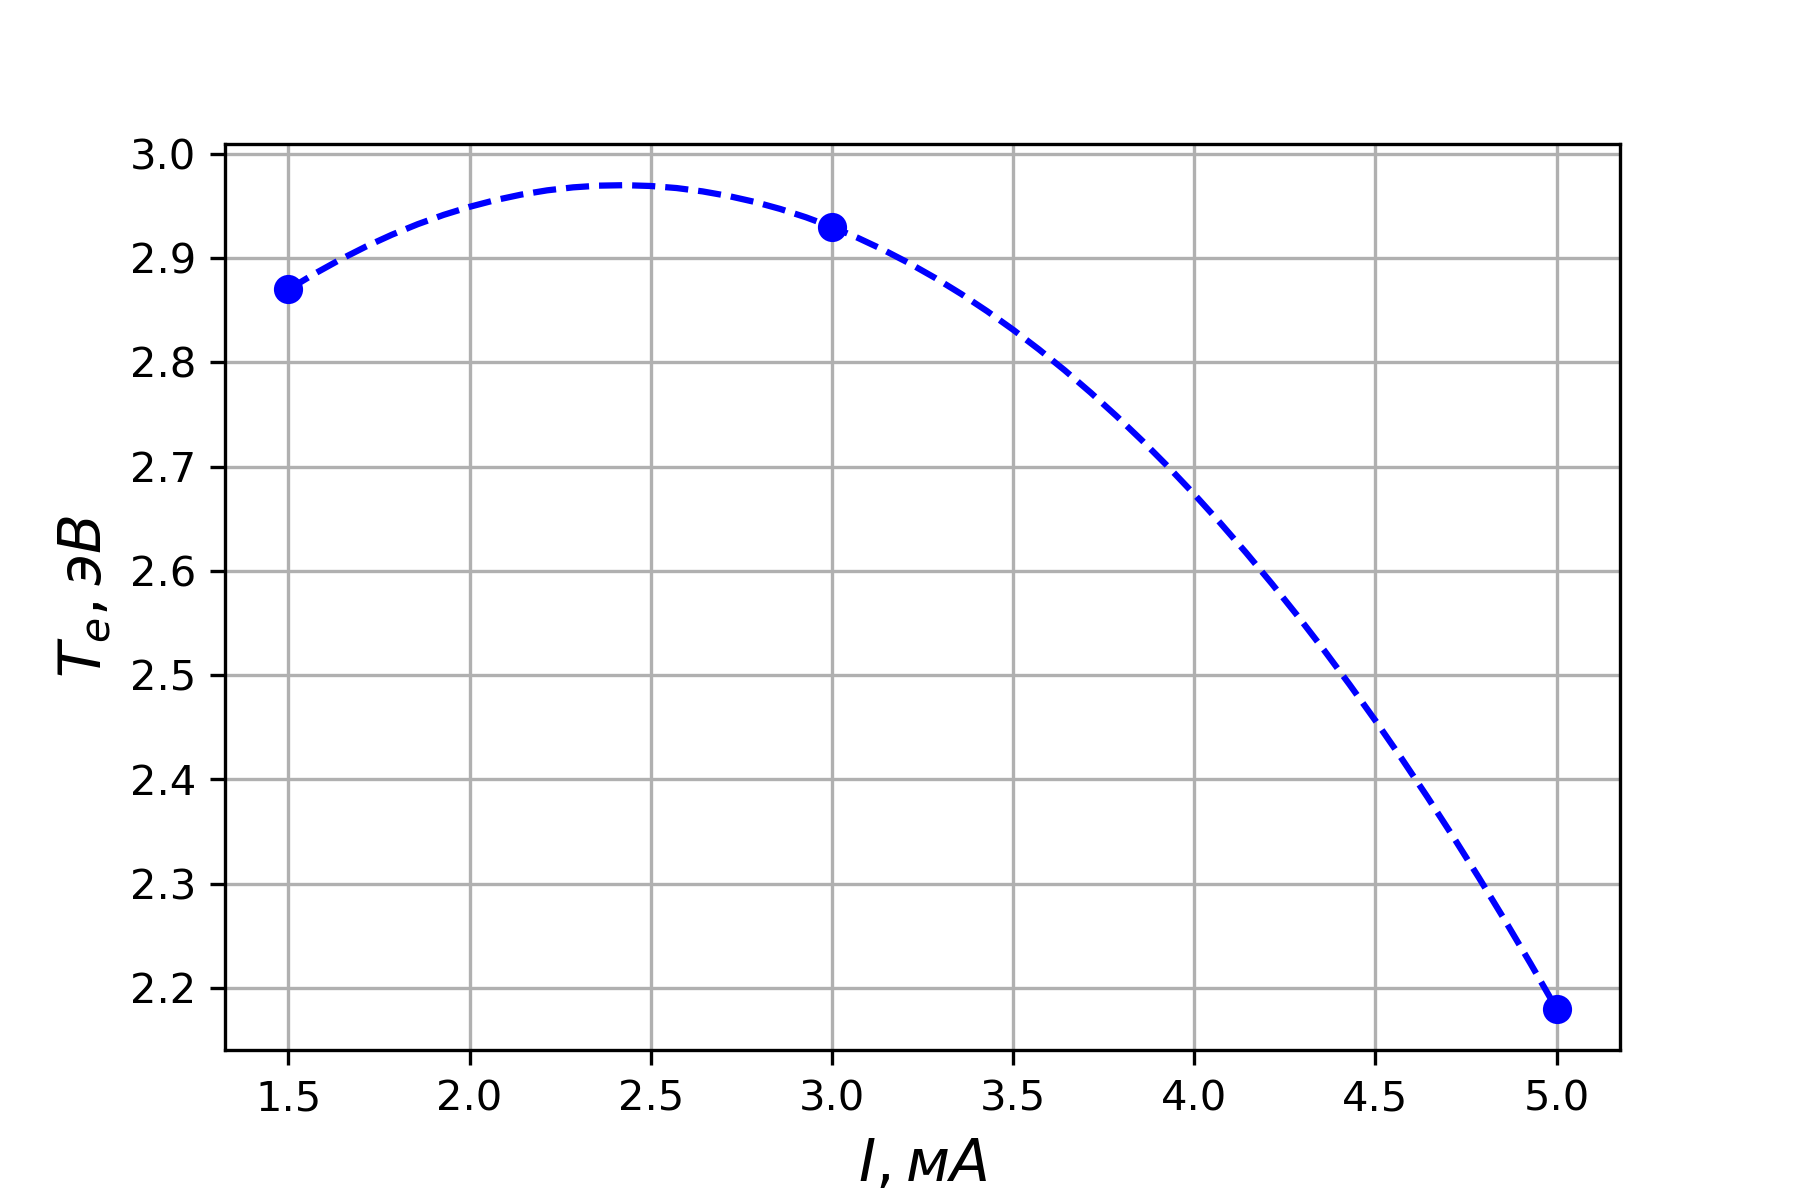
\includegraphics{T_e(Ip).png}
\end{center}
\caption{Зависимость $T_e(I)$}
\label{T_e(I)}
\end{figure}

\end{document}